\chapter{Material Layering in Unreal and Unity}\label{cha:implementationParametricLayering}

\emph{UE4} as well as \emph{Unity} include different approaches on how to work with material layering. The chapter starts with an introduction of how \emph{Epic} designed their node based shading model for \emph{UE4} to work for material layering. This is an interesting point if you consider implementing a shading model yourself or if you want to get a better understanding of shading models in other software. The chapter continues by explaining which systems already exist in order to create layered materials within the engines, how to access them and how they work. The use cases, advantages and disadvantages of the individual systems are described later in the design patterns category (see chapter \ref{cha:patterns}).  

 

\section{\emph{UE4} A Shading System for Material Layering}

In \emph{UE4}, the ability to create a simple and efficient material layering system was an essential requirement when recreating the shading model for the \emph{UE4}. This shading system uses a simplified and adopted model of the \emph{Disney's} principled BRDF \cite{burley2012physically} to fit the requirements of a real-time engine \cite[p.\,9]{karis2013real}. The unification of the shader model allows the recreation of most real world materials by sharing the same parameters across all shaders. This is a fundamental point for creating an efficient pattern layering workflow as already mentioned in section \ref{sec:patternLayering}. The \emph{UE4} developer removed some advanced shading techniques (e.g., subsurface scattering, transparency, clear coat) from the standard shading model. For optimization reasons, they implemented individual shader models for those special cases. They simply expanded them by some additional features.  As these shading models are almost identical, it is easy to change the shading model of a shader later on.

Adaptations of the principled BRDF shading system are widely implemented in a vast variety of other 3D packages such as the \emph{Substance Suite} \cite[p.\,8]{wes2018comprehensivevol1}, \emph{Blender} \cite{blender2017bsdf}, \emph{Marmoset Toolbag} and many more. Using similar input parameters for the shading system makes a production pipeline between different softwares possible. Materials can be previewed, created and manipulated in other softwares with minor changes in the material inputs (e.g., textures and vertex attributes). Due to minor differences in the implementation, it might be necessary to adapt the textures and material inputs to achieve identical visual results. The \emph{Substance Suite} includes presets to export the textures properly for the target applications like\emph{UE4}. All modifications are stored in presets and can therefore simply be exported when exporting the textures.        

One simplification done in the shading model of \emph{UE4} was to treat advanced shader instructions like subsurface scattering, anisotropy, clearcoat and sheen as special cases, separately from the standard shading model. This was done to minimize the performance overhead. The base shading model for \emph{UE4} contains base color, metallic, roughness and cavity \cite[p.\,9--10]{karis2013real}. To the best of my knowledge, the cavaty parameter is not an explicit input parameter in the \emph{UE4} shader but rather a generated cavity map based on the the normal map.\,This cavity map is used to create small scale shadows that could not be produced by regular real-time shadows. This cavity map is then multiplied onto the base color and the specular value. The specular value is set to 0.5 by default which represents a constant f0\footnote{Fresnel zero defines the percentage of specular light that is reflected on a surface directly facing the camera \cite[p.\,10]{wes2018comprehensivevol1}.} value of 0.04 for non dielectric materials \cite{epic2018physicalMaterial}. This value can be overwritten by the specular input.    

	
\section{Material Layering Implementation}\label{sec:patternLayeringInUEUnity}

Both game engines---\emph{UE4} as well as \emph{Unity}---support different ways of working with material layering. One method provided by both engines is to create custom shaders using the shading language Cg/HLSL \cites{unity2017ShaderLanguague,epic2018shader}. Writing custom shader code requires much experience and time but provides the most control. Additionally, both engines offer other tools to customize shaders, for example the shader graph editors. They provide access to a huge library of shader operation and input nodes. The system automates a lot of the optimization work and creates automatically optimized shader code in the background. Working in a node based workflow makes creating custom shaders more accessible and user-friendly. This allows even less experienced users with less technical background to create complex shaders. \emph{UE4} provides two additional systems to support and streamline material layering. These systems provide a workflow to increase re-usability, flexibility and efficiency. They are mainly workflow systems. Identical visual results could also be achieved by using any of the other methods mentioned here. Figure \ref{fig:ComparisonRocketLayering} shows a simple example that was recreated identically by using different approaches.  

\subsection{Node Based Shader Graphs}
Both real-time engines---\emph{Unity} and \emph{UE4}---provide a node based way of authoring shaders (see figure \ref{fig:shadergraphs}). These powerful tools provide access to a huge amount of shader operations, functions and inputs that can be used to create custom shaders as well as layered material shaders. Both systems are flexible enough to create layered material shaders using several base materials and complex masking and blending operations. The node based design makes it easy and fast to iterate on shaders and adopt them constantly to the project needs. All examples and tests were performed by using these shader graphs and the specific layered material systems built on top of them (see section \ref{sec:matLayV1} and section \ref{sec:matLayV2}).  

\begin{figure}
	\centering\small 
	\begin{tabular}{@{}cc@{}}
		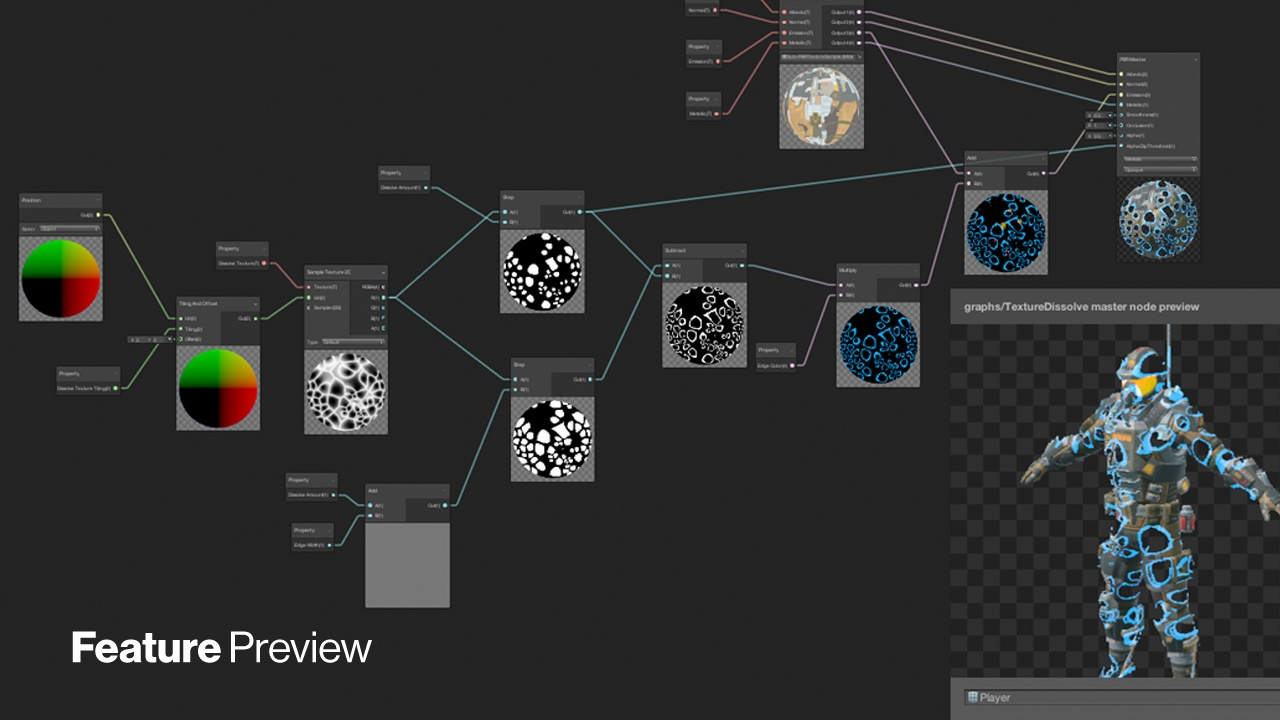
\includegraphics[width=0.475\textwidth]{images/05cha_01_unityShaderGraph.jpg} &		% JPEG file
		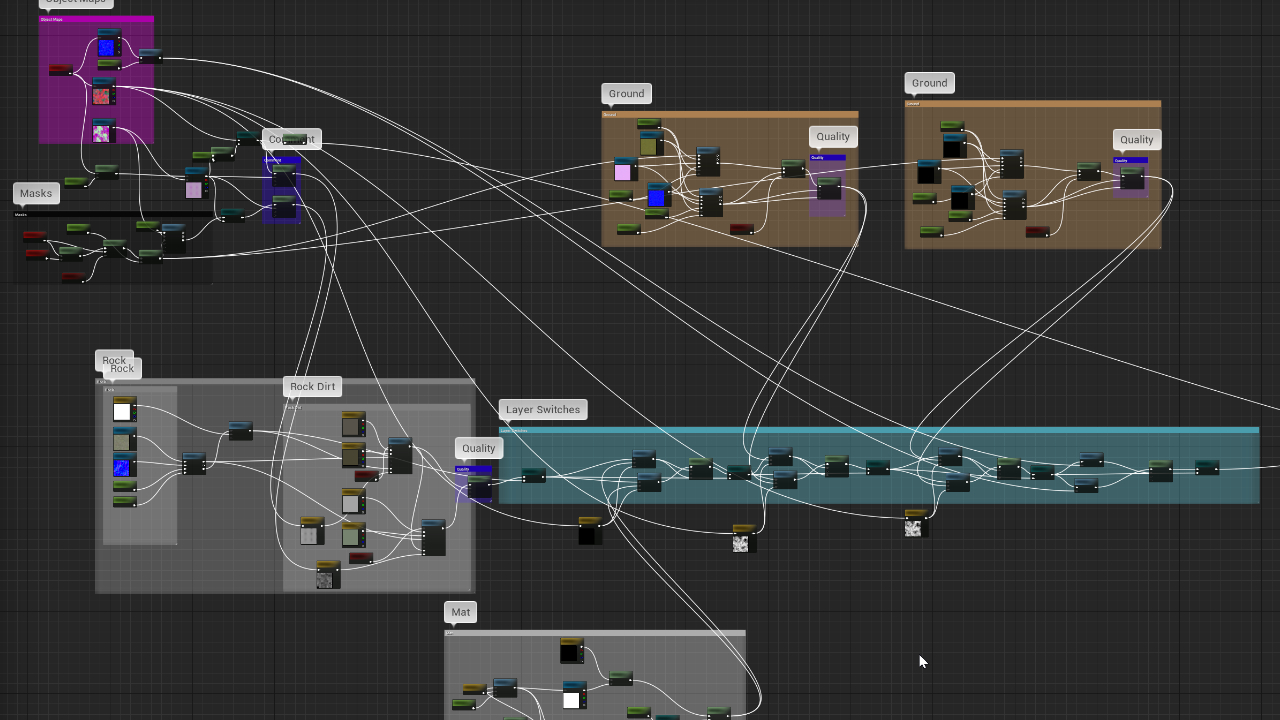
\includegraphics[width=0.475\textwidth]{images/05cha_01_shaderGraphUE_02.jpg} \\	% PNG file
		(a) & (b) 
	\end{tabular}
	\caption{\emph{Unitys} shader graph editor (a) and \emph{UE4} material editor (b).
		Both engines, \emph{Unity} and \emph{UE4}, include a node based editor to create and manipulate custom shaders. Image source: \cite{cooper2018visualEditor}. }
	\label{fig:shadergraphs}
\end{figure}


\subsection{\emph{UE4} Material Layering V1}\label{sec:matLayV1}
The first material layering system was implemented as an extension of the pre-existing material function\footnote{ Material functions are parts of a shader graph that can be saved as independent sub-graphs. They can contain complex shader graph networks. Material functions can be reused across different shader graphs, stored in libraries and shared amongst artists.} system \cite{epic2015LayeredMats}. 
The different parameters (base color, roughness, metallic, etc.) of a base material---a material container---can be combined into one node by using the \emph{Make Material Attributes} node. This can be thought of as a container including all parameters necessary to describe the surface properties of a material. All parameters of the base material are now handled as a single output. This material container or layer can also be easily moved out into a self contained sub-graph (a material function) and be referenced into any other shader graph. The architecture of these material functions allows reusing them as many times as wanted. This works for all kinds of different shaders. Single material layers can be blended together in different ways by using pre-defined \emph{Material Layer Blend} functions. They provide different blending modes and operations for splitting, combining and manipulating single parameters. Section \ref{sec:blendingModule} discusses the issue of blending single material attributes. It also shows how material layering system can support the artist in blending them properly. In one of \emph{Epic's} live streams introducing the newer material layering system \cite{unreal2018materialLayering}, Alan Willard, Lauren Ridge and Chris Bunner summarize the most important shortcomings of the material layering system v1:

\begin{description}
	\item [Clarity:] Creating a master material using many different layers can end up in a huge graph which might be difficult to understand at a later point in the project. This issue becomes more urgent the more layers are added and the more material instances and different combinations of layers are needed. 
	\item [Flexibility:] Adding a new layer or layer variation for certain objects result in the need to update the shader graph. This can either be done by using static switches or adding the changes to a new copy of the shader. The former results in a growing node tree. Every change in the shader graph results in a re-evaluation of all material instances. The latter results in big number of different shaders. Changes and optimizations are not automatically propagated to all materials and need to be added manually to all shader graphs if not contained within a material function. A growing complexity within the shader graph of an increasing number of shader graphs decreases flexibility and simplicity. 
	\item [Functions:] The material layering system relies on material functions and therefore shares the issue of this system, like the difficulty in passing on parameters. Parameters need to be explicitly exposed from the material function to be accessible from the surrounding shader. Parameters cannot be exposed directly from the material function to the parameter windows of the material instances.      
\end{description}


\subsection{\emph{UE4} Material Layering V2}\label{sec:matLayV2}

The new material layering system represents an entirely new workflow. The same results could be achieved with prior methods, but ease of use, flexibility and clarity have been improved hugely. The material layering system has been streamlined and split into different components: the \emph{Material Layers} and \emph{Material Layer Blends} \cite{epic2015materialLayers}. This represent a logical separation between defining a layer and blending the independent layers. A \emph{Material Layer} is a material container defining a base material using an independent shader graph. \emph{Material Layer Blends} handles the blending between two arbitrary input materials by defining masking as well as blending. The architecture of the \emph{Material Layering V2} is similar to the schematic high level description presented in chapter \ref{cha:partsOfLayeredShader}.  A \emph{Material Layer} object in \emph{UE4} is equal to the concept of a material container. The \emph{Material Layer Blend} includes both the blending module as well as the masking container. 

In the old system, replacing a base material, cobblestone ground with concrete or simply adding a new layer, would result in the need to add an additional base material into the shader graph. As mentioned before, this introduces new switches and a growing shader graph. Alternatively, a modified copy of the shader could be created. Anyway, this results in an increasingly complex shader graph and the re-evaluation of all material instances using this shader. 
In the new system a base material layer can simply be swapped out without any need for manual change or the re-evaluation of all material instances. This is possible because the material containers are not specified by the shader. The material layering system creates the shader dynamically based on the used\emph{ Material Layers} and \emph{Material Layer Blend}s. This logical separation of layer definition and layer blending eliminates most of the former shortcomings mentioned in the section before, such as flexibility, clarity  and the need to re-evaluate all material instances. 


\begin{figure}
	\centering\small 
	\begin{tabular}{@{}ccc@{}}
	\multicolumn{3}{c}{
\includegraphics[width=0.9\textwidth]{images/05cha_02_LayeredMaterials.jpg}} \\
	\multicolumn{3}{c}{(a)} \\
	[6pt]	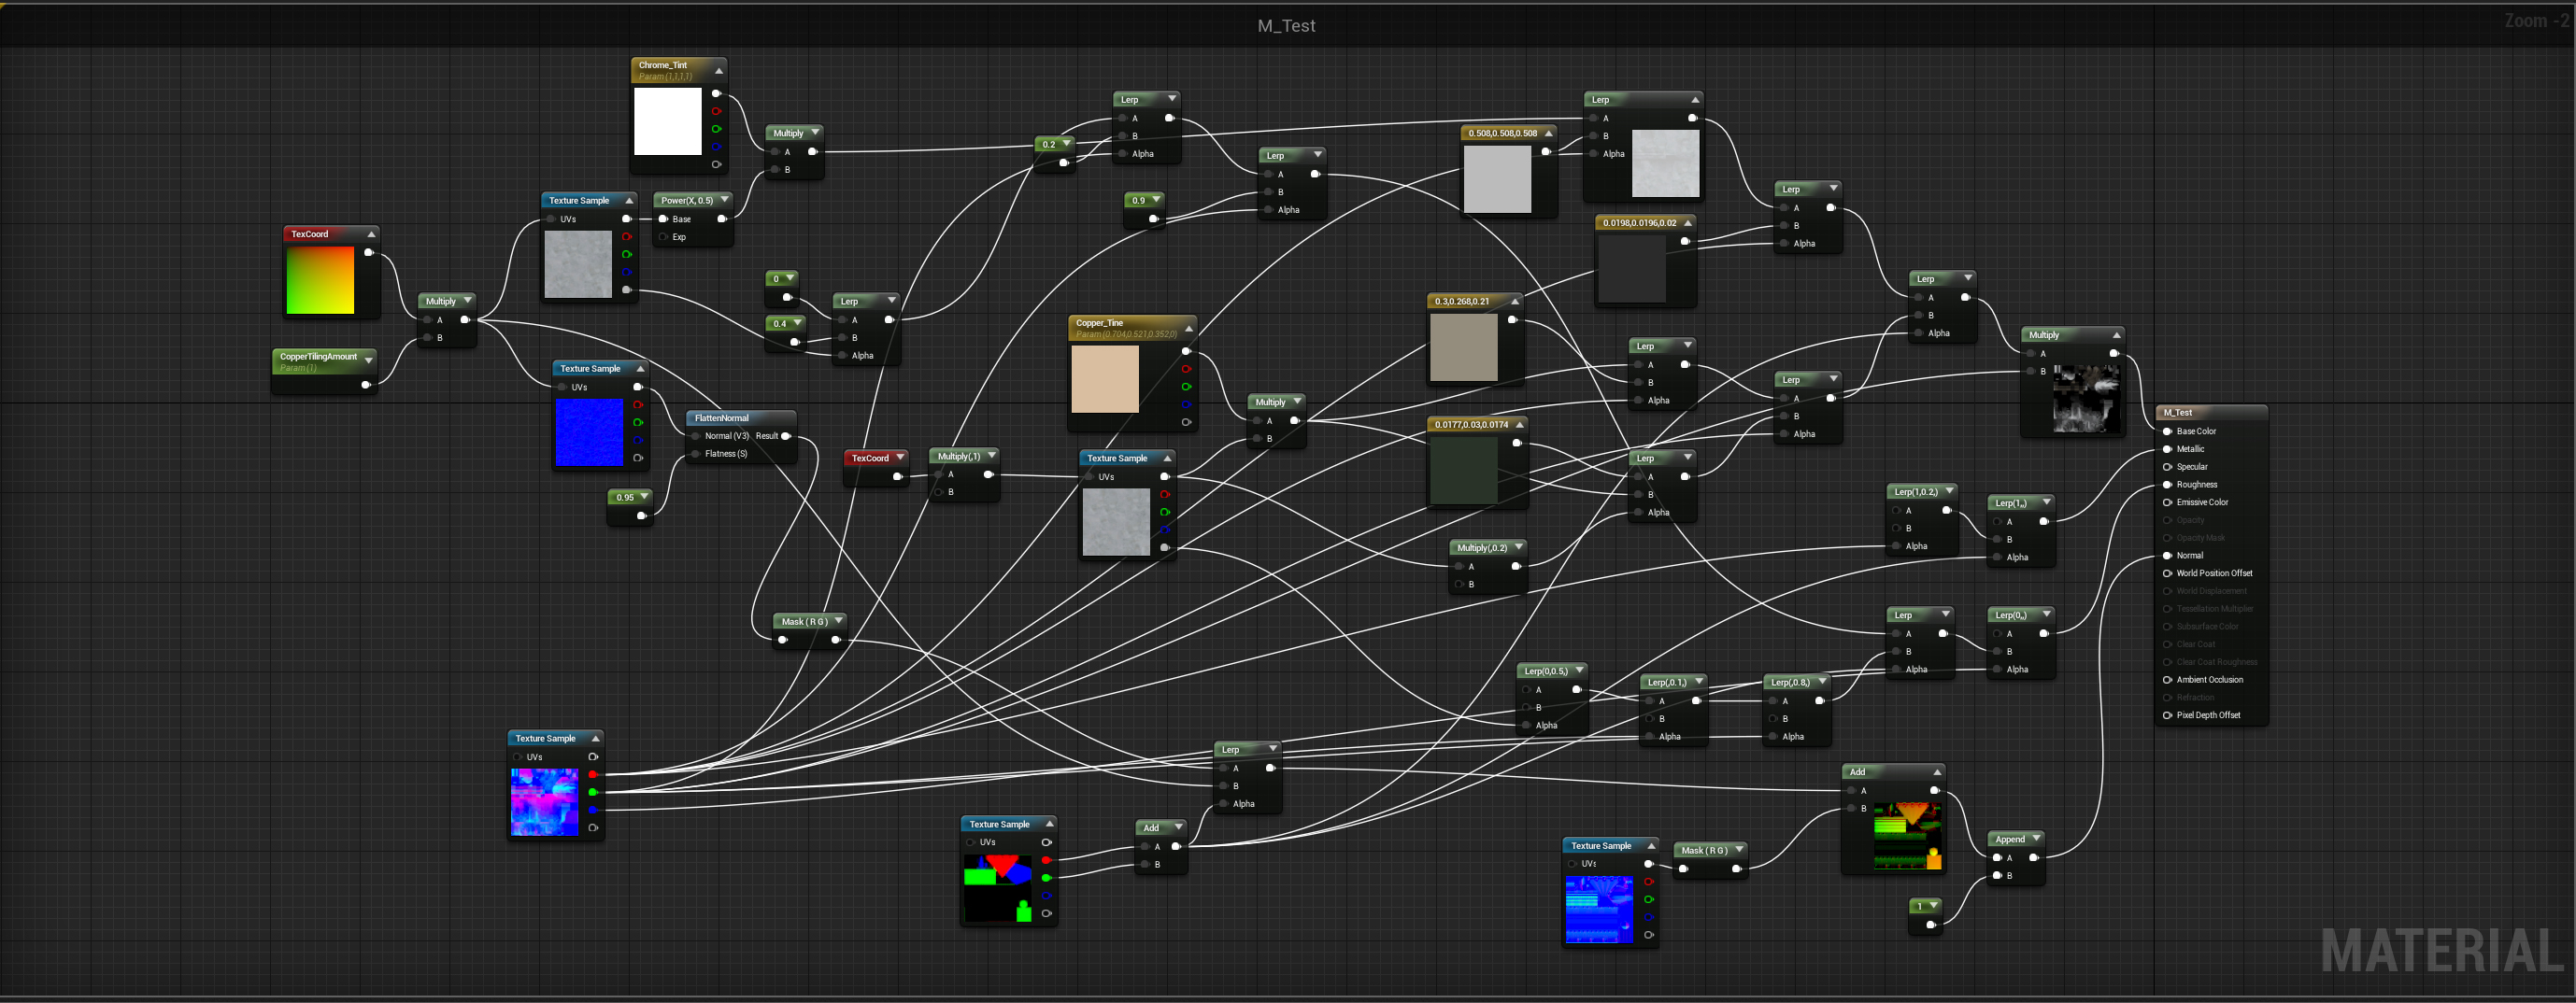
\includegraphics[width=0.39\textwidth]{images/05cha_02_ue4_Rocket_Material_Beforelayers.jpg} &
	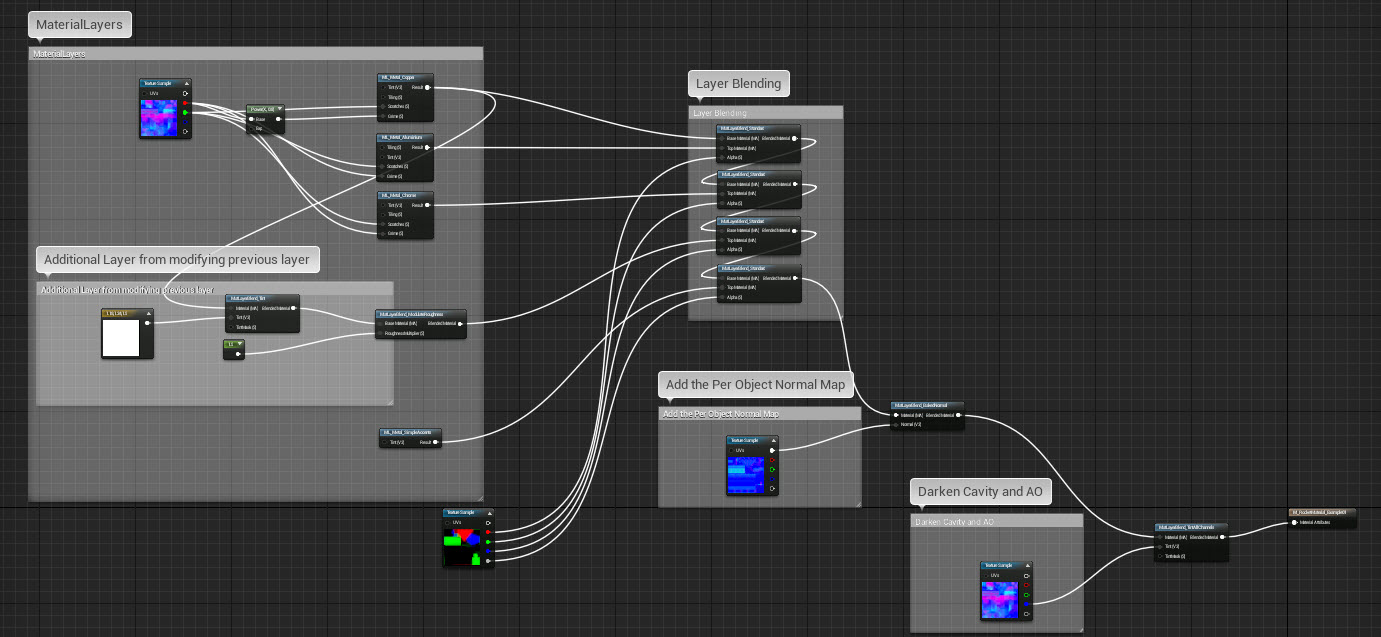
\includegraphics[width=0.33\textwidth]{images/05cha_02_ue4_MatieralLayering.jpg} &
	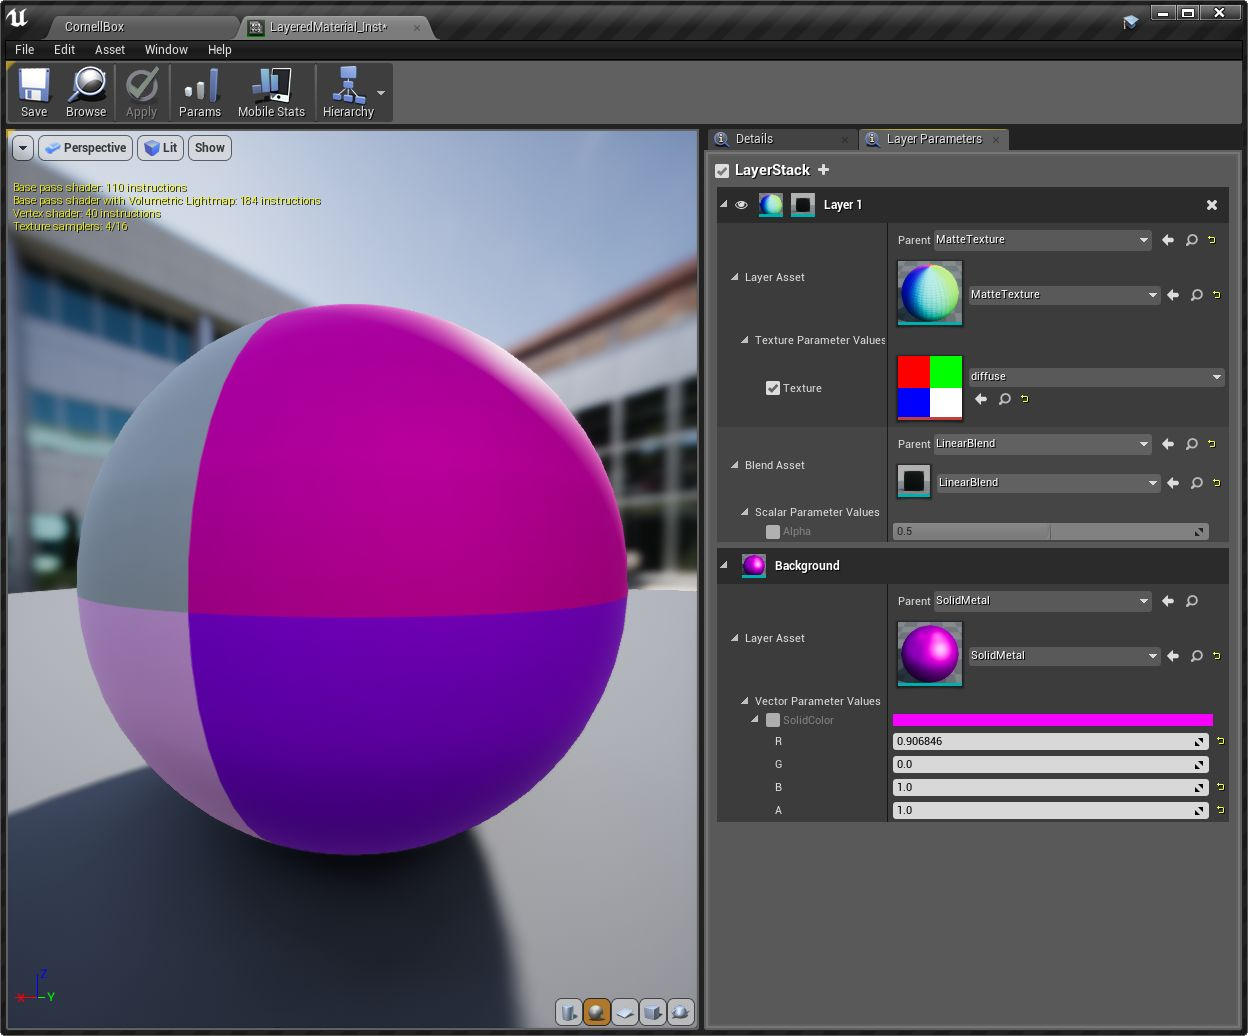
\includegraphics[width=0.19\textwidth]{images/05cha_02_MaterialLayerInstance_RN.jpg}	\\
	(b) & (c) & (d)
	\\[6pt]	
	\end{tabular}

	\caption{Identical visual result from different pattern layering systems. Figure (a) shows the final object using material layering. Figure (b) shows a shader graph setup without using material layers. The example on figure (c) shows the shader graph using the \emph{Material Layering V1}. As comparison, figure (d) shows the UI for the the \emph{Material Layering V2} system. Image sources: \cites{epic2015materialLayers,pesare2017material}.}
	\label{fig:ComparisonRocketLayering}
\end{figure}


\subsection{Pre-existing Layered Material Shaders}\label{sec:preexistingShaders}

\emph{Alegorithmic}---a software developer specialized on texture authoring tools---provides a layered material shader for \emph{Unity} and \emph{UE4} that can be downloaded from \emph{Substance Share} website.\footnote{Download for \emph{UE4} \url{https://share.allegorithmic.com/libraries/2125} and \emph{Unity }\url{https://share.allegorithmic.com/libraries/2126}).} This shader allows the blending of five or ten base materials that are all defined exclusively by texture inputs. Additionally, it supports objects specific textures like normal map and ambient occlussion. 
These shaders are not a blackbox. In both game engines \emph{Unity} and \emph{UE4} the shader code or the shader graph setup can be modified. Hugely modified versions of this material were used for some of the layered shaders in the project \emph{Letzte Worte}.

\emph{Unity} gets shipped with a layered shader called \emph{LayeredLit} as a part of the \emph{HDRenderPipeline} package. This shader is designed for environment assets created by using photogrammetry. Nevertheless, this shader could also be used for any other kind of asset. Creating an efficient, flexible and easy to use shader affords much time, expertise and testing. Using this pre-existing layered shader can therefore be really useful. The shader code is included in the \emph{HDRenderPipeline} package and can easily be adopted and modified to fit the specific project needs. 

\section{Summary}

An interesting aspect of this chapter is how \emph{Epic} already considered material layering  when redesigning its node base shading graph system for \emph{UE4}. An important step hereby was to standardize the shading model. It uses the same shader parameters across all materials. For performance optimizations they introduced variations of the shading model supporting advanced features (e.g., subsurface scattering, translucence, clear coat). The individual shaders can easily be adopted to fit another shading model. The second important step was to use algorithms that propagate in a linear and proportional way. Especially as regards the roughness value,  this solves the issue of wrong roughness accumulation on an engine level.
\emph{Unity} as well as \emph{UE4} implement different methods to use material layering. Both enginges support custom shaders---written in Cg/HLSL---and powerful in engine shader graph editors. On top of this node based shading system, \emph{UE4} implemented two dedicated systems to improve the material layering workflow. Before passing on to material layering design patterns, I want to examine the approaches of other authors to develop such catalogs for decision making.  


